\chapter{Dettagli implementativi}

In questo capitolo verranno descritti i pattern principali usati durante la progettazione e lo sviluppo del software e le motivazioni che hanno portato a tali scelte.

\section{Custom container controller}
Il \emph{Container View Controller} è un pattern di progettazione iOS che permette di scomporre le applicazioni in parti più piccole e semplici, ognuna delle quali è dedicata ad assolvere un determinato compito. I container controller sono usati quindi come intermediari tra queste diverse parti (\emph{child controller}) allo scopo di fornire un'interfaccia che sia coerente con il contesto in cui i controller figli operano.

\begin{figure}[!htbp]
\centering
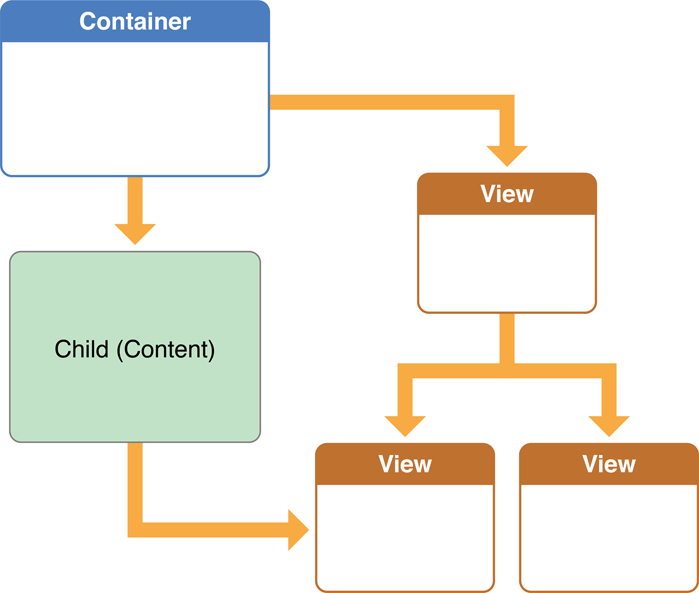
\includegraphics[scale=0.30]{architettura/container.png}
\caption{Schema del \emph{contaier controller design}}
\label{fig:selettore}
\end{figure}

L'utilizzo di tale pattern ha permesso durante la progettazione dell'applicazione di ottenere controller più puliti sotto il punto di vista implementativo ed efficienti sotto il punto di vista delle prestazioni.

\subsection{MiaSituazioneContainerController}
\label{parag:miasituaz}
Uno dei requisiti funzionali principali dell'applicazione prevede la visualizzazione dei conti e delle carte di un utente e l'eventuale visualizzazione dei movimenti ad essi relativi.

La parte dell'architettura elaborata per realizzare tali funzionalità è composta dalla seguente gerarchia di container e child controller:

\begin{itemize}
 \item MiaSituazioneContainerController (figura \ref{fig:miasituazione}): è il container controller che ha il compito di creare l'interfaccia di base e di creare un array di child controller:
 \begin{itemize}
  \item ContiContainerController: è il container che gestisce la creazione e la comunicazione tra i controller adibiti alla visualizzazione dei prodotti bancari come vista a bolle o vista a tabella (nello specifico \emph{BubbleViewController} e \emph{ContiTableViewController})
  \item MovimentiContainerController: è il container che gestisce la creazione e la comunicazione tra i controller adibiti alla visualizzazione dei movimenti di un determinato conto (nello specifico \emph{TimelineViewController} e \emph{MovimentiTableViewController})
  \item ContiFilterTableViewController: il controller che si occupa della visualizzazione e della logica di filtraggio dei conti che l'utente può visualizzare sullo schermo
 \end{itemize}
\end{itemize}
\begin{figure}[!htbp]
\centering
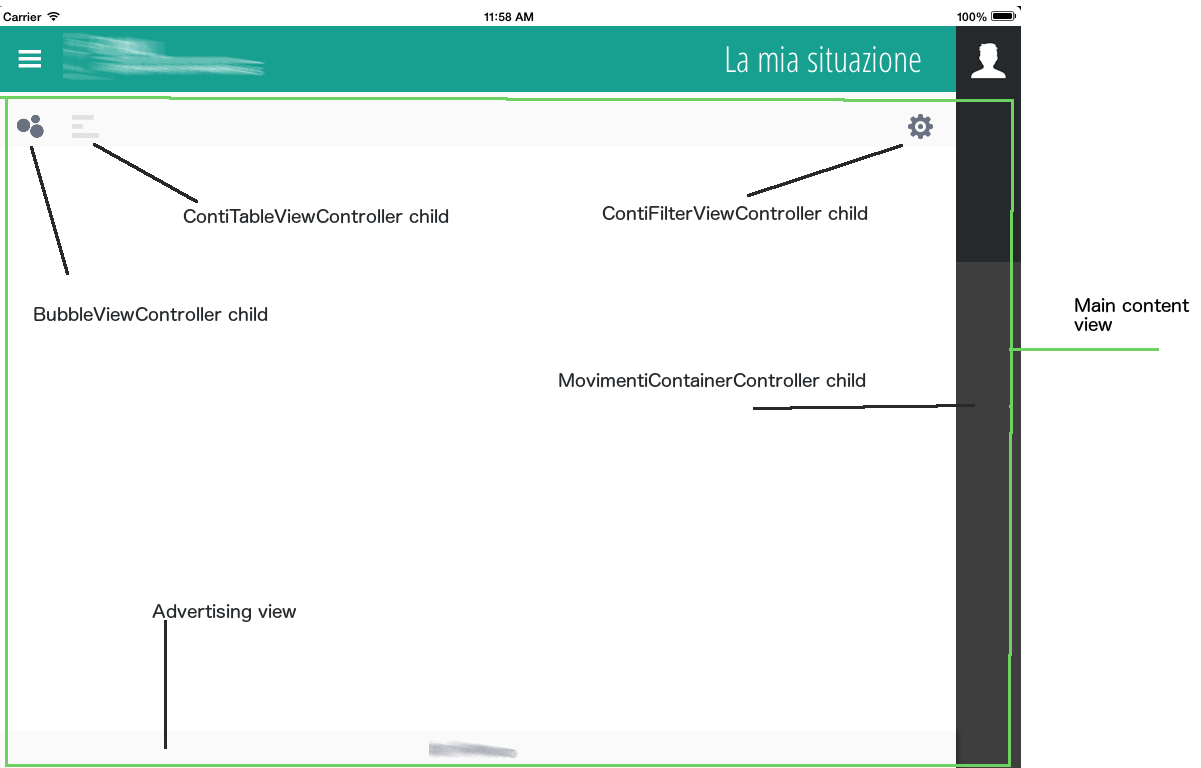
\includegraphics[scale=0.35]{dettagli/miasituazione.png}
\caption{Dettaglio componenti gestiti da MiaSituazioneContainerController}
\label{fig:miasituazione}
\end{figure}
\begin{figure}[!htbp]
\centering
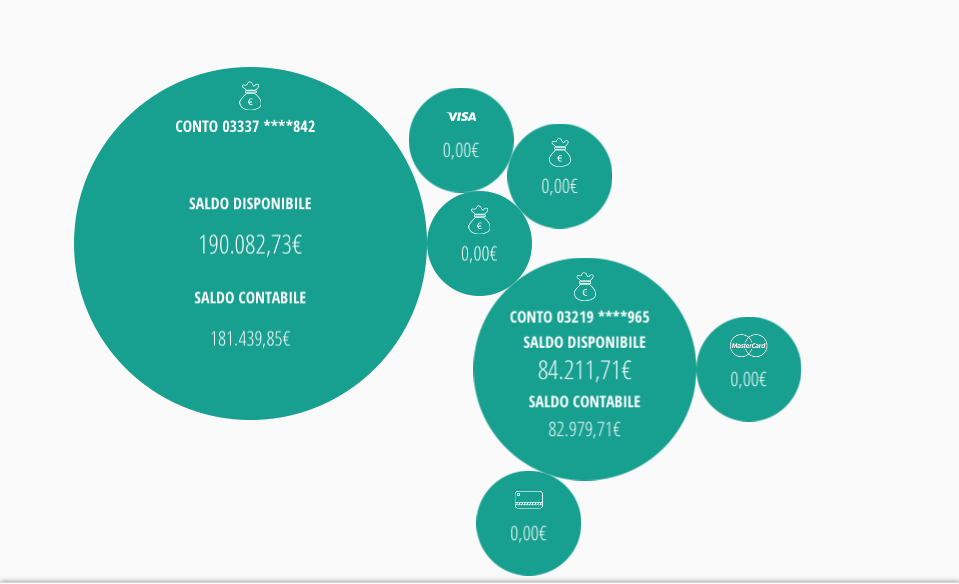
\includegraphics[scale=0.35]{dettagli/bubble.png}
\caption{BubbleViewController}
% \label{fig:miasituazione}
\end{figure}
\begin{figure}[!htbp]
\centering
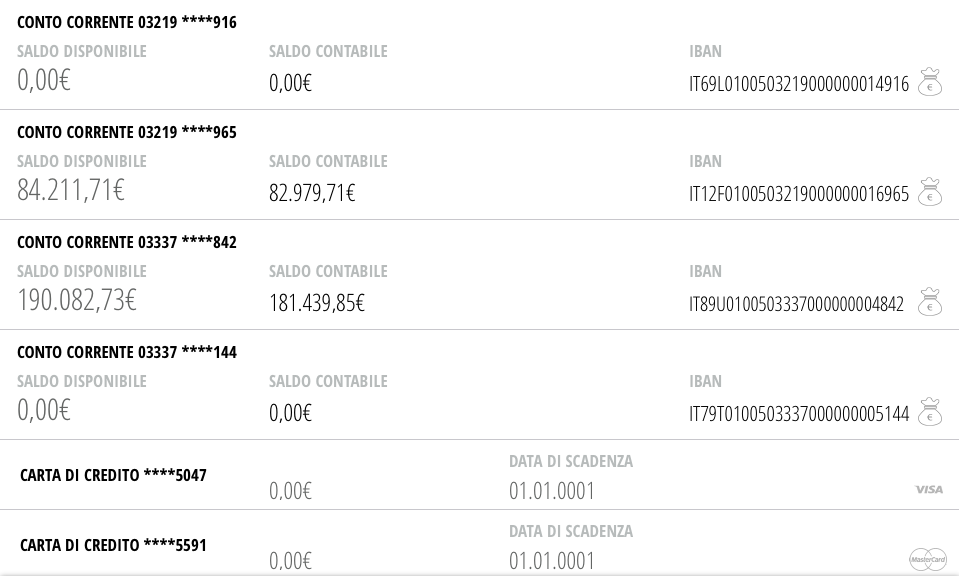
\includegraphics[scale=0.35]{dettagli/contiList.png}
\caption{ContiTableViewController}
% \label{fig:miasituazione}
\end{figure}
Quando \emph{MiaSituazioneContainerController} viene istanziato, è eseguita una chiamata ai servizi per ottenere la lista dei conti dell'utente, tale lista verrà quindi utilizzata come model comune a tutta la gerarchia dei controller descritti sopra. È compito quindi del MiaSituazioneContainerController gestire gli eventi dell'interfaccia principale e passare il model a uno dei controller figli quando l'utente sceglierà una delle modalità di visualizzazione descritte precedentemente. 

\subsection{MovimentiContainerController}

Come brevemente descritto nel paragrafo \ref{parag:miasituaz} tale container ha il compito di gestire i child controller adibiti alla visualizzazione dei movimenti di un conto. 
Nello specifico tale container si occupa della gestione ad alto livello delle funzioni e degli eventi relativi ai componenti dell'interfaccia da esso gestiti (figura \ref{fig:movimenticontainer}). A titolo illustrativo esso gestisce gli eventi scatenati dal selettore dei conti e dal filtro calendario; in particolare ad ogni cambio di conto o di data del filtro il MovimentiContainerController effettua una chiamata ai servizi per ottenere una lista di movimenti che verrà utilizzata come model comune a tutti i figli di tale container.

\begin{figure}[!htbp]
\centering
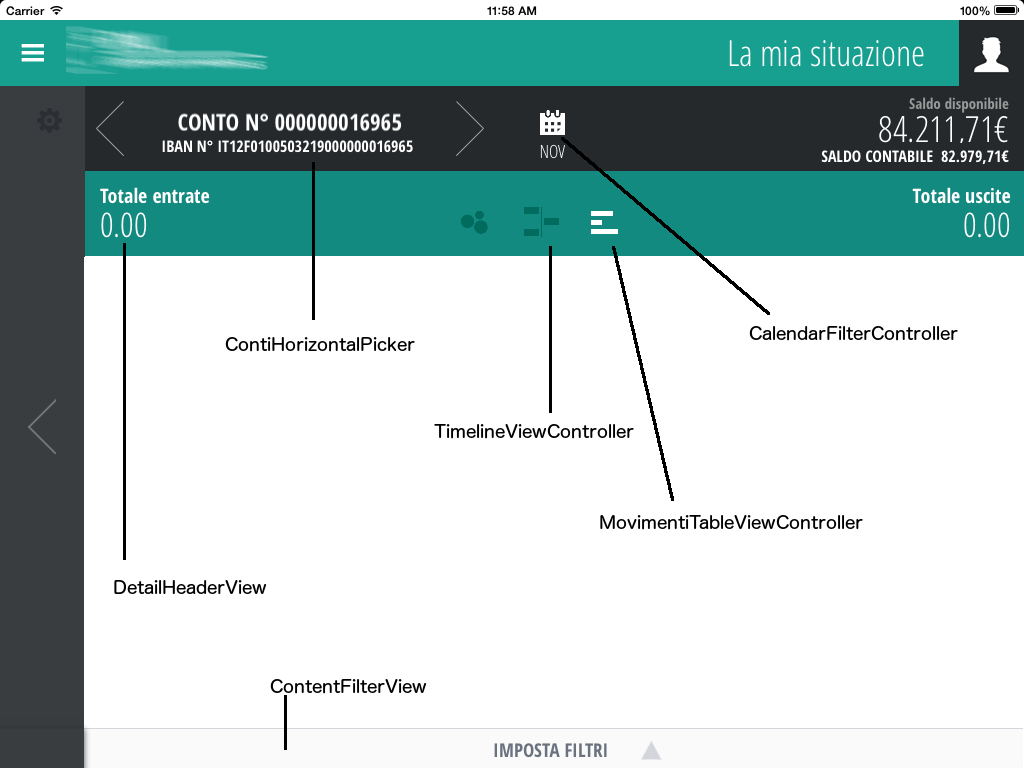
\includegraphics[scale=0.35]{dettagli/movimenticontainer.png}
\caption{Dettaglio dei componenti gestiti dal controller MovimentiContainerController}
\label{fig:movimenticontainer}
\end{figure}

\subsection{Comunicazione tra container e child controller}
I container controller sono gli unici componenti consapevoli dell'esistenza di altri controller nella gerarchia, in particolare dei child controller da loro direttamente creati.
I child controller sono realizzati quindi come componenti indipendenti che non hanno percezione del controller padre o dei loro fratelli. 

La comunicazione tra i container e i suoi figli è stata realizzata in modo tale da garantire sempre un'elevata modularità dell'architettura mediante l'utilizzo dei pattern messi a disposizione dall'SDK iOS:

\begin{itemize}
 \item message passing: realizza la comunicazione in avanti tra un container e un child controller mediante opportune interfacce messe a disposizione dai child contoller
 \item pattern delegate: realizza la comunicazione all'indietro da un child ad un container controller mediante la dichiarazione di opportuni protocolli (\emph{protocol} nella tecnologia iOS) da parte dei child controller. I container controller vengono quindi dichiarati conformi a tali protocolli e posti come \emph{delegate} ( oggetti che operano come aiutanti adibiti all'esecuzione di compiti particolari)
\end{itemize}

L'adozione di tali pattern durante la progettazione ha permesso di ottenere un'architettura modulare composta da componenti specializzati facilmente estendibili e riusabili.

\begin{figure}[!htbp]
\centering
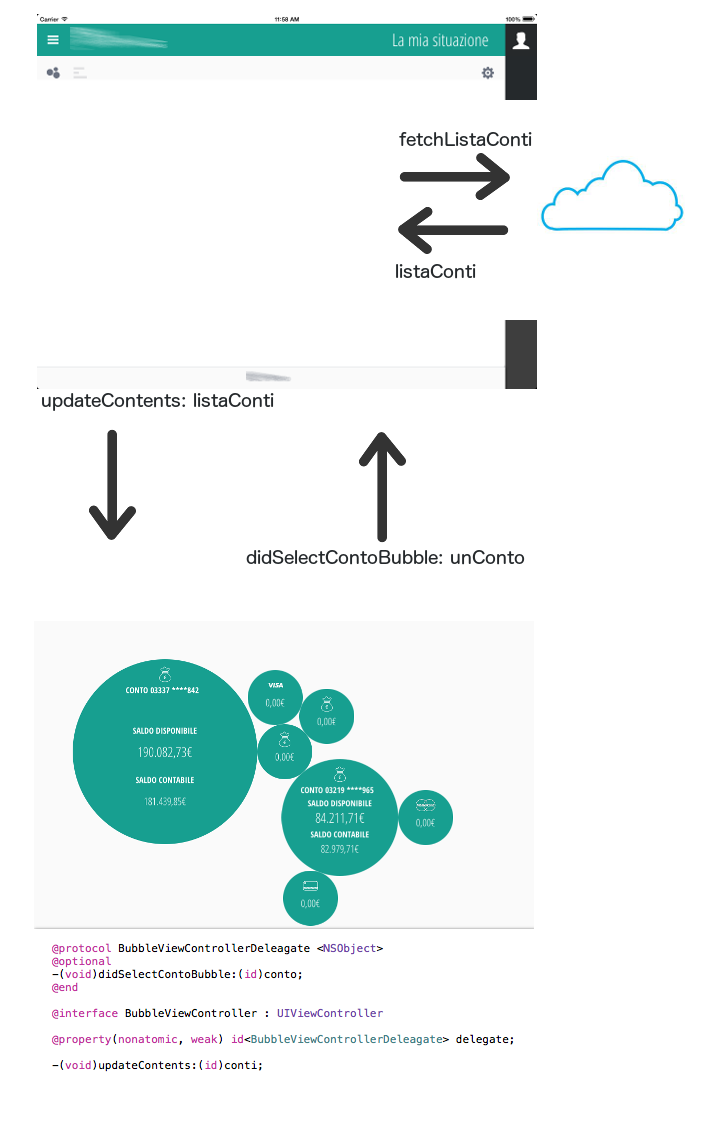
\includegraphics[scale=0.6]{dettagli/communication.png}
\caption{Esempio di comunicazione da un container padre a un child controller}
\label{fig:comunicazione}
\end{figure}

\newpage
\section{Posizionamento di oggetti in uno spazio cartesiano}
All'interno dell'applicazione è stato realizzato un algoritmo per il posizionamento di oggetti grafici in uno spazio cartesiano. Tali oggetti sono visualizzati come circonferenze all'interno dell'interfaccia grafica e sono utilizzati per riassumere i dati di un conto corrente o di una carta di credito (come importo, tipo di conto, ecc\dots).

La visualizzazione delle circonferenze ha dovuto rispettare i seguenti vincoli:

\begin{itemize}
 \item  devono esser visualizzate il più possibile una vicino all'altra
 \item  non si devono sovrapporre
 \item  non  devono uscire da nessun lato dello schermo 
 \item 	devono esser tutte visibili
\end{itemize}

\subsection{Realizzazione}

Per non bloccare l'interfaccia grafica durante il calcolo, l'esecuzione dell'algoritmo di posizionamento avviene in un thread asincrono così da non occupare il \emph{main thread} e lasciare quindi la libertà all'utente di continuare ad utilizzare l'applicazione.

Nei prossimi paragrafi saranno illustrati gli oggetti e le logiche utilizzate per realizzare l'algoritmo e rispettare i vincoli descritti precedentemente.

\subsubsection{Bubble}

La documentazione Apple suggerisce di non effettuare il disegno e l'allocazione di oggetti grafici (oggetti che estendono la classe \texttt{UIView}) al di fuori del main thread, in quanto può portare a problemi di thread safety. Per questo motivo è stata realizzata la classe \texttt{Bubble} che ha il compito di astrarre un oggetto view e di incapsulare solo le sue proprietà geometriche (come la dimensione, l'origine, il centro, ecc\dots). L'algoritmo sfrutterà quindi gli oggetti Bubble per effettuare il calcolo del posizionamento nello spazio.

Per decidere in quale punto dello spazio posizionare una circonferenza e per decidere in quale punto su di essa posizionare un vicino, ogni oggetto Bubble calcola le seguenti proprietà:
\begin{itemize}
 \item frame: rappresenta l'origine e la dimensione di una bubble
 \item center: le coordinate del centro di una bubble
 \item radius: il raggio
 \item anchorPoints: un array di oggetti \texttt{AnchorPoint}
\end{itemize}

\subsubsection{AnchorPoint}

La classe \texttt{AnchorPoint} rappresenta le coordinate $(x,y)$ di un punto su una circonferenza. Tale oggetto è utilizzato per decidere in quale posizione di una bubble aggiungere un'altra bubble (figura \ref{fig:anchor}). 

\begin{figure}[!htbp]
\centering
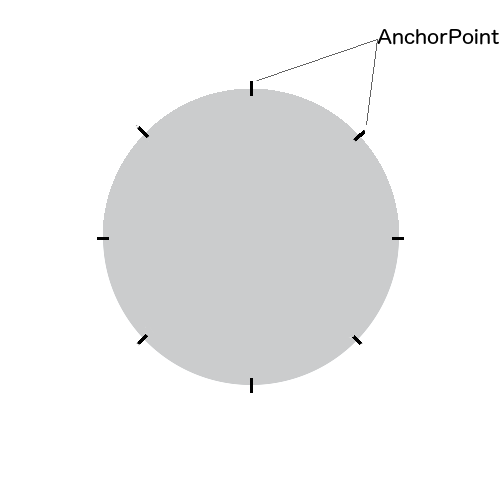
\includegraphics[scale=0.4]{dettagli/anchor.png}
\caption{Esempio di AnchorPoint su una circonferenza}
\label{fig:anchor}
\end{figure}

\subsubsection{Algoritmo}
Di seguito saranno descritte in pseudo-codice le procedure che compongono l'algoritmo di posizionamento.
\\\\
La computazione inizia richiamando la procedura \ref{algo:1} che calcola la dimensione di ogni bubble in base al saldo di un conto e controlla se tali bubble entrano  nell'area delimitata dall'interfaccia grafica, altrimenti esegue un ridimensionamento e riesegue ricorsivamente il calcolo.
\begin{lstlisting}[label=algo:1,caption=startBubblesAlgorithm,breaklines=true]

startBubblesAlgorithm(float resizePercent){
    
    //sizesArray contiene le dimensioni di tutte le Bubble calcolate
    
    for each(conto in contiList){
	bubbleSize = calculateBubbleSizeForConto(conto)
	add bubble to sizesArray
    }
  
    bool isGood = checkArea(sizesArray)
    
    if(isGood){
      createBubbles
      placeBubblesInSpace
    }
    else{
	startBubblesAlgorithm(0.1)
    }
}


\end{lstlisting}

Verificato che le bubble entrano nell'area viene richiamata la procedura \ref{algo:2} la quale lancia il calcolo delle posizioni degli oggetti Bubble all'interno dell'area delimitata dall'interfaccia. Questo calcolo viene ripetuto fino a quando non viene trovata una disposizione ideale per gli oggetti. Al termine della computazione verranno creati gli oggetti \texttt{BubbleView} che saranno successivamente disegnati all'interno dell'interfaccia grafica.

% delle posizioni degli oggetti Bubble all'interno dell'area delimitata dall'interfaccia. In particolare la procedura prova una posizione per ogni bubble, in caso positivo viene lanciato il disegno su schermo, altrimenti viene eseguito un ridimensionamento delle bubble e viene rilanciato l'algoritmo per il posizionamento. per  Questo calcolo viene ripetuto fino a quando non si trova una disposizione ideale delle circonferenze. Al termine della computazione verranno creati gli oggetti \texttt{BubbleView} che saranno successivamente disegnati all'interno dell'interfaccia grafica.
\begin{lstlisting}[label=algo:2,caption=placeBubblesInSpace,breaklines=true]

placeBubblesInSpace{
    
    bool finished = false
    
    while(finished == false){
    
	//calcola la posizione per ogni Bubble
	calculateOriginForBubbles
	
	//se non ha avuto successo
	if(recalculate){
	
	    //pulisce le strutture dati create dai calcoli precedenti
	    cleanOldData 
	    //ricrea gli oggetti Bubble con ridimensionamento
	    resizeValue += 0.1
	    createBubbles 
	}
	else{
	  finshed = true;
	}
    }
    
    //disegna sull'interfaccia le BubbleView ottenute dalle Bubble
    drawBubbleViewInSpace
}


\end{lstlisting}


La procedura \texttt{calculateOriginForBubbles} (listato \ref{algo:3}) inizia posizionando la prima Bubble al centro dello schermo. Nei passi successivi cerca di posizionare le restanti bubble considerando, per ogni Bubble già posizionata, i suoi AnchorPoint e controllando se ne esiste uno utilizzabile: cioè un punto su una Bubble tale che affiancandogli un'altra Bubble quest'ultima non esca dai lati dallo schermo o si sovrapponga alle altre già posizionate. Se tale punto esiste la Bubble viene considerata come \emph{posizionata} e l'anchorPoint \emph{occupato}, altrimenti vengono controllati iterativamente gli AnchorPoint di tutte le restanti Bubble già posizionate. Trovato un anchorPoint valido vengono calcolate le coordinate $(x,y)$ che formeranno il centro della nuova bubble da visualizzare. Queste coordinate giacciono sulla retta che congiunge l'anchorPoint trovato e il centro della bubble che lo contiene (\ref{fig:bubblesInView}).

Questo meccanismo permette di sfruttare tutta l'area a disposizione ricontrollando iterativamente gli spazi che avanzano dopo il posizionamento di una Bubble, in modo tale da ottenere una distribuzione uniforme degli oggetti.

\newpage
\begin{figure}[!htbp]
\centering
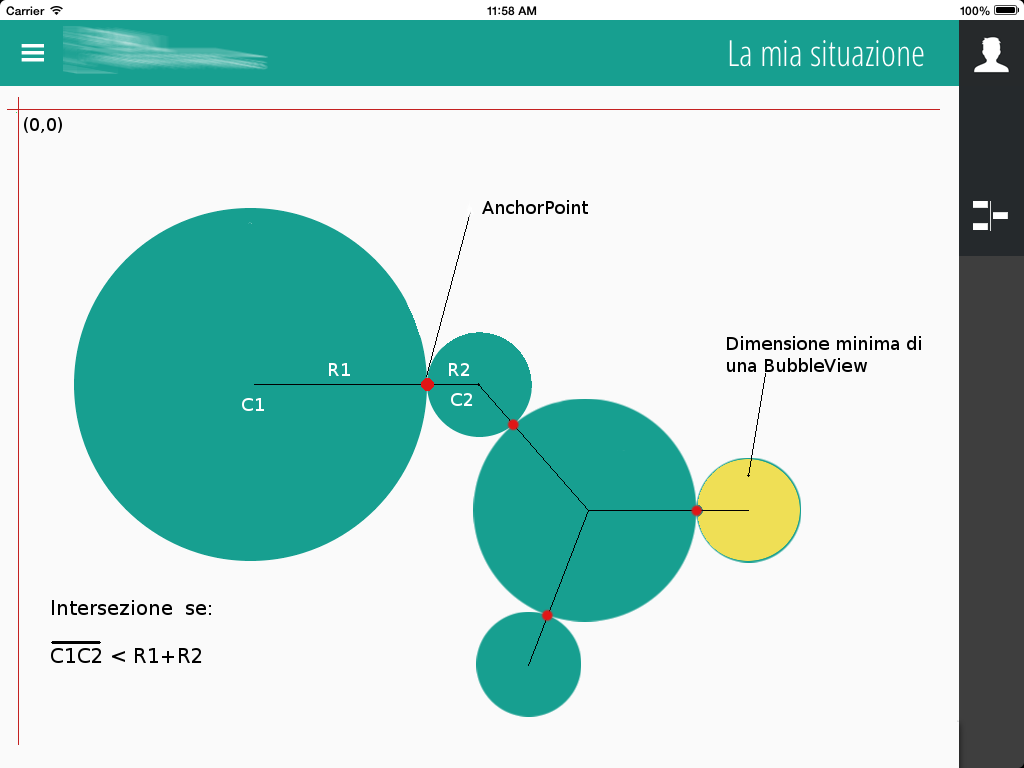
\includegraphics[scale=0.4]{dettagli/bubblesInView.png}
\caption{Dettaglio del calcolo delle posizioni}
\label{fig:bubblesInView}
\end{figure}

\begin{lstlisting}[label=algo:3,caption=calculateOriginForBubbles,breaklines=true,  commentstyle=\color{CadetBlue}]
calculateOriginForBubbles{

    //bubbles è l'array di oggetti Bubble per i quali deve esser calcolato il posizionamento
  
    for each(newBubble in bubbles){

        BOOL isFound = NO;

        //se prima bolla
        if(newBubble isFirst){
	    newBubble.center = view.frame.center
            add newBubble to placedBubbles
            continue;
        }

        BOOL intersect = NO;

        //cerco posizione per newBubble tra gli anchor point delle bubble già posizionate
        for(bubble in placedBubbles){

            //controllo anchorPoint di bubble
            for each (anchorPoint in bubble){

                //un punto di ancoraggio
                anchorPoint = bubble.getRandomAnchorPoint

                if(anchorPoint.isBusy){
		    //se occupato salto ciclo
                    continue;
                }

                intersect = NO;

                //provo con questo punto
                //calcolo il centro dove posizionare la newBubble rispetto l'anchorPoint selezionato e il centro ad esso relativo
                aCenter = calculateCenter(bubble.center,point.angle,newBubble.radius + bubble.radius)

                newBubble.center = aCenter;

                //salto se con questa posizione si esce sotto, sopra o a sinistra dello schermo
                if(exit from screen){
                    continue;
                }

                //termino se esce a destra dello schermo
                if(aCenter.x + newBubble.radius > screenFframe.size.width)
                    recalculate = YES;
                    return;
                }

                //controllo se newBubble si interseca con le altre view già posizionate
                for(bubble2 in placedBubbles){

                    if (bubble != bubble2){
	    
                        distance = distanceFrom:bubble2.center,aCenter);
                        extendedRadius = newBubble.radius + bubble2.radius;

                        //se distanza tra due centri è minore della somma dei raggi, si intersecano
                        if( distance < extendedRadius){
                            //si intersecano
                            intersect = YES;
                            break;
                        }
                    }
                }
                
                //se finito ciclo allora newBubble non si interseca con nessun'altra bubble
                if(intersect == false){
                    //segno come occupato l'anchor point in esame
                    point.isBusy = true;
                    isFound = true;
                     //interrompo controllo degli altri anchor point
                    break;
                }
            }

            if(isFound ){
                //interrompe ricerca sulla prossima bolla tra quelle inserite
                break;
            }
        }

        if(!isFound){
            //Arriva qui se ha finito tutti gli anchor point di tutte le bolle già inserite.
            recalculate = YES;
            return;
        }

        //se arrivato qui aggiunge newBubble alle già  posizionate
        add newBubble to placedBubbles
    }
}
\end{lstlisting}


\subsection{Prestazioni}
Dalle analisi effettuate sulla base di dati del sistema bancario è stato osservato che il numero di conti e delle carte posseduto in media da ogni cliente è minore o uguale a dieci.

L'algoritmo creato, pur effettuando ad ogni iterazione il controllo di tutti gli AnchorPoint di ogni Bubble posizionata, mantiene ottime prestazioni visualizzando gli oggetti in una ridotta frazione di secondi. Per questo motivo è stato ideato anche un meccanismo di ricalcolo delle posizioni basato sul ridimensionamento degli oggetti Bubble nel caso in cui in una istanza di calcolo non si trovi una disposizione ottimale degli oggetti.  
In particolare, quando l'algoritmo fallisce, riprova a calcolare le posizioni scalando la dimensione degli oggetti e rilanciando il posizionamento. Il ridimensionamento è stato realizzato diminuendo di una certa percentuale il diametro delle Bubble. Per permettere la visualizzazione almeno del saldo e dell'icona del prodotto bancario, il ridimensionamento delle Bubble può essere effettuato purché il loro diametro non sia inferiore a una determina lunghezza.
\\\\
Inoltre, per evitare di eseguire l'algoritmo ogni volta che l'utente apre la pagina relativa alla \emph{La Mia Situazione}, è stato realizzato il caching dei dati relativi alle posizioni delle bubble all'interno dell'interfaccia. Questo ha permesso di velocizzare ulteriormente la navigazione tra una pagina e un'altra dell'applicazione.

\section{Grafico a bolle}

Per permettere la visualizzazione dei grafici a bolle sono state estese le funzionalità del framework \texttt{CorePlot}, in particolare sono state realizzate delle classi che modificano il grafico \emph{CPTScatterPlot} cioè la classe che premette il disegno di grafici a barre.

In tale grafico le barre sono state ridisegnate come bolle, in cui le ascisse di ogni bolla del grafico indicano le date dei dati da rappresentare, le ordinate indicano i saldi di ogni elemento e il diametro delle bolle è data una funzione dipendente dal saldo e dai valori delle dimensioni massime e minime secondo la seguente formula:



%  bubbleDiameter = (((point.y) * (MAX\_DIAMETER - MIN_DIAMETER)) / (_max))+MIN_DIAMETER;

% \begin{displaymath}
% \newcommand{\bcdot}{\boldsymbol{\cdot}}
% 
% \begin{multiline}
%  $bubbleDiameter = \biggl({point.y \bcdot (MAX\_DIAMETER - MIN\_DIAMETER)  \over max }\biggr) \\ + MIN\_DIAMETER $
% \end{multiline}

\begin{align}
%   \phantom{i + j + k}
  &\begin{aligned}
%     \mathllap{a} &= b + c + d\\
%       &\qquad + e + f + g + x + y + z
      bubbleDiameter = \biggl({point.y \times (MAX\_DIAMETER - MIN\_DIAMETER)  \over max }\biggr) \\ + MIN\_DIAMETER
  \end{aligned}
\end{align}

% \end{displaymath}

Dove $point.y$ indica il valore del saldo della i-esima bolla, $MAX\_DIAMETER$ e $MIN\_DIAMETER$ indicano rispettivamente il diametro massimo e minimo che una bolla può assumere e $max$ rappresenta il valore massimo presente nell'insieme dei dati da rappresentare nel grafico.
In questo modo è stato possibile ridimensionare le bolle in modo tale da non occupare troppo spazio all'interno dello schermo e ottenendo quindi una visione omogenea dei dati.
\\\\
Per disegnare le etichette verticali su ogni bolla è stata realizzata la seguente procedura:

//creo la label
    

    

    //array delle coordinate del punto plottato
    NSDecimal plotPoint[2];

    //valore della x
    NSNumber *plotXvalue = [self numberForPlot:plot

                                         field:CPTScatterPlotFieldX

                                   recordIndex:index];

    plotPoint[CPTCoordinateX] = plotXvalue.decimalValue;

    

    //valore della y
    NSNumber *plotYvalue = [self numberForPlot:plot

                                         field:CPTScatterPlotFieldY

                                   recordIndex:index];

    plotPoint[CPTCoordinateY] = plotYvalue.decimalValue;

    

    //valore y del punto da plottare

    CPTXYPlotSpace *plotSpace = (CPTXYPlotSpace *)_graph.defaultPlotSpace;

    

    // esegue conversione dalle coordinate del dato alle coordinate dello spazio cartesiano del grafico

    CGPoint dataPoint = [plotSpace plotAreaViewPointForPlotPoint:plotPoint numberOfCoordinates:2];

    

    // convert from plot area coordinates to graph (and hosting view) coordinates

    //centro del cerchio nella view hosting

    dataPoint = [_graph convertPoint:dataPoint fromLayer:_graph.plotAreaFrame.plotArea];

    

    

    //punto della VIEW su cui attaccare la label

    CGFloat labelYorigin = dataPoint.y+(bubbleDiameter/2)+15;

    

    //debug view

    //UIView *ciao = [[UIView alloc] initWithFrame:CGRectMake(dataPoint.x, labelYorigin, 2, 2)];

    //ciao.backgroundColor = [UIColor greenColor];

    //[self.hostingView addSubview:ciao];

    //

    

    //calcolo il VALORE dell'offset tra il centro del cerchio e il punto dove deve esser disegnata la label nel sistema di riferimento del grafico

    NSDecimal labelPlotPoint[2];

    CGPoint dataPointExtended = CGPointMake(dataPoint.x, labelYorigin-dataPoint.y + textLabelWidth);

    [plotSpace plotPoint:labelPlotPoint numberOfCoordinates:2 forPlotAreaViewPoint:dataPointExtended];

    //[plot.plotSpace plotPoint:labelPlotPoint forPlotAreaViewPoint:dataPointExtended];

    

    //l'offset da aggiungure al centro del cerchio nel sistema di riferimento del grafico

    float offset = [[NSDecimalNumber decimalNumberWithDecimal:labelPlotPoint[CPTCoordinateY]] floatValue];

    

    //NSLog(@"\n saldo = %f,\n label sopra il saldo = %f",point.y, point.y + offset);

    

    

    

    CGFloat x = point.x;

    NSNumber *anchorX = [NSNumber numberWithFloat:x];

    

    CGFloat y = point.y + offset + diameterValue;

    NSNumber *anchorY = [NSNumber numberWithDouble:y];

    

    CPTPlotSpaceAnnotation *priceAnnotation = [[CPTPlotSpaceAnnotation alloc] initWithPlotSpace:plot.plotSpace anchorPlotPoint:[NSArray arrayWithObjects:anchorX, anchorY, nil]];

    priceAnnotation.rotation = M_PI /2;

    

    

    priceAnnotation.contentLayer = textLayer;

    

    [plot.graph.plotAreaFrame.plotArea addAnnotation:priceAnnotation];
